\documentclass[tikz,border=5pt]{standalone}
\usepackage{luatexja}
\usepackage[hiragino-pron]{luatexja-preset}
\usepackage{amsmath,amssymb}
\usepackage{pgfplots}
\pgfplotsset{compat=1.18}
\usetikzlibrary{arrows.meta,patterns}

\begin{document}
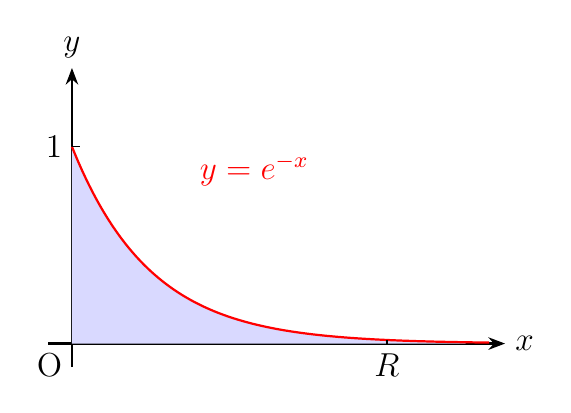
\begin{tikzpicture}[every node/.style={font=\large}]
  % Axes
  \draw[-{Stealth[length=6pt]}, thick] (-0.3,0) -- (5.5,0) node[right] {$x$};
  \draw[-{Stealth[length=6pt]}, thick] (0,-0.3) -- (0,3.5) node[above] {$y$};

  % Shaded region
  \fill[blue!15, domain=0:5, samples=100]
    (0,0) -- plot (\x, {2.5*exp(-\x)}) -- (5,0) -- cycle;

  % Curve y = e^{-x}
  \draw[thick, red, domain=0:5.3, samples=200] plot (\x, {2.5*exp(-\x)});

  % R line
  \draw[dashed, thick] (4,0) -- (4,{2.5*exp(-4)});

  % Labels
  \node[below] at (4,0) {$R$};
  \node[left] at (0,2.5) {$1$};
  \draw[dashed] (0,2.5) -- (0.1,2.5);
  \node[right, red] at (1.5,2.2) {$y = e^{-x}$};

  % Origin
  \node[below left] at (0,0) {O};
\end{tikzpicture}
\end{document}
